\chapter{Implementation Details}
% This is where you explain what you have implemented and how you have implemented it. Place here all the details that you consider important, organize the chapter in sections and subsections to explain the development and your workflow.\\Given the self-explicative title of the chapter, readers usually skip it. This is ok, because this entire chapter is simply meant to describe the details of your work so that people that are very interested (such as people who have to evaluate your work or people who have to build something more complex starting from what you did) can fully understand what you developed or implemented.\\Don't worry about placing too many details in this chapter, the only essential thing is that you keep everything tidy, without mixing too much information (so make use of sections, subsections, lists, etc.). As usual, pictures are helpful.

\section{Tools used for the Chrome extension}

Extensions are made of different, but cohesive, components. Components can include background scripts, content scripts, an options page, UI elements and various logic files. Extension components are created with web development technologies: HTML, CSS, and JavaScript. An extension's components will depend on its functionality and may not require every option.

In this project the extension was build with the following tools:

\begin{itemize}
    \item HTML
    \item CSS
    \item Typescript
    \item Node
    \item React
    \item Webpack
    \item Material-UI
\end{itemize}

Let's see in the details each of these tools.

\subsection*{HTML}

As said in the previous section, the extension is made with the web development technologies. HTML, HyperText Markup Language, is one of them.
In this project, HTML does not have a central role, since it is managed automatically by webpack. However, when the extension is build, the popup and the options main page are in HTML. 

\subsection*{CSS}

    CSS, Cascading Style Sheets, is another web development technology. In this project, CSS is lightly used to style the extension's UI. The majority of the styling part is done through React and Material-UI. However, it's important to mention CSS, since it heavily used and is a key part of the web development workflow.

\subsection*{Typescript}

    Typescript is a web development technology that is used to write code in a more readable and easy to understand way. In this project, Typescript is used to write the extension's logic.
    Typescript is a syntactic superset of Javascript and adds optional static typing to the language. Another difference compared to Javascript is that Typescript is compiled and not interpreted. This means that the extension will not run unless it is compiled. The reason behind the creation of Typescript was the maintenance of large-scale applications. So the decision of using Typescript was made to make the extension's code more maintainable. 
    In addition, since Typescript has a static typing system, that enables static language analysis, which simplifies the devolopment process by providing meaningful errors.
\subsection*{Node}

Node.js is an open-source, cross-platform, back-end JavaScript runtime environment that runs on the V8 engine and executes JavaScript code outside a web browser
Node.js has an event-driven architecture capable of asynchronous I/O. These design choices aim to optimize throughput and scalability in web applications with many input/output operations, as well as for real-time Web applications (e.g., real-time communication programs and browser games).
Node.js allows the creation of Web servers and networking tools using JavaScript and a collection of "modules" that handle various core functionalities.

npm is the pre-installed package manager for the Node.js server platform. It installs Node.js programs from the npm registry, organizing the installation and management of third-party Node.js programs. Packages in the npm registry can range from simple helper libraries to task runners.

\subsection*{React}

React (also known as React.js or ReactJS) is a free and open-source front-end JavaScript library for building user interfaces based on UI components. It is maintained by Meta (formerly Facebook) and a community of individual developers and companies. React can be used as a base in the development of single-page, mobile, or server-rendered applications with frameworks like Next.js. However, React is only concerned with state management and rendering that state to the DOM, so creating React applications usually requires the use of additional libraries for routing, as well as certain client-side functionality.

\subsection*{Webpack}

Webpack is a free and open-source module bundler for JavaScript. It is made primarily for JavaScript, but it can transform front-end assets such as HTML, CSS, and images if the corresponding loaders are included. Webpack takes modules with dependencies and generates static assets representing those modules.

% Insert image
\begin{figure}[h!]
    \vspace{0.5cm}
    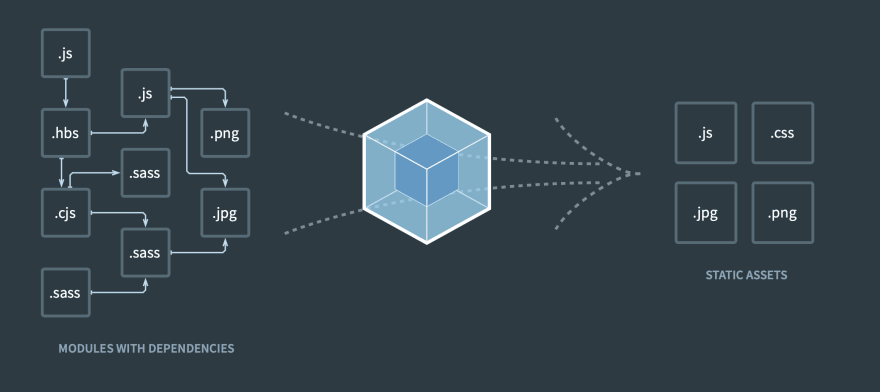
\includegraphics[width=\textwidth]{images/webpack-bundle.png}
    \caption{Webpack workflow}
    \label{fig:webpack-bundle} % This is the image label, with which you can refer to the image in any document location.
\end{figure}

\subsection*{Material-UI}

Material UI is an open-source React component library that implements Google's Material Design. In this project is used to create the extension's UI.
It includes a comprehensive collection of prebuilt components that are ready for use in production right out of the box.
Material UI is beautiful by design, and features a suite of customization options that make it easy to implement your own custom design system on top of our components.
The main advantages of material UI are:

\begin{itemize}
    \item Ready to use
    \item Follow Google's Material Design so it is consistent with a big part of the web
    \item Realiable with a great community
\end{itemize}


\section*{Design Choices}

In this section all design choices are explained. For each key part of the extension there is an image showing it and there is a complete explanation. 
